\documentclass{beamer}

\usepackage[utf8]{inputenc}
\usepackage[russian]{babel}
\usepackage{graphicx}

\usetheme{Madrid}


\title[ВКР]
{Гамильтонов формализм для задачи гарантированного синтеза управлений при геометрической неопределенности}

\author[Е. В. Гуров]
{студент 4 курса Е. В. Гуров \\
научный руководитель --- академик, д.ф.-м.н., проф. А. Б. Куржанский}

\institute[СА]
{ Кафедра системного анализа \\
факультета ВМК МГУ имени М.В. Ломоносова}

\date[28 апреля 2022 г.]

\begin{document}

\frame{\titlepage}

\begin{frame}{Постановка задачи}

Рассматривается система
\begin{equation*}
    \dot{x} = A(t)x + B(t)u + C(t)v(t)
\end{equation*}
с непрерывными по \( t \) матрицами \( A(t), B(t), C(t) \).
\begin{itemize}
    \item \( x \in \mathbb{R}^n \) --- вектор состояния системы
    \item \( u \in \mathbb{R}^p \) --- управление
    \item \( v \in \mathbb{R}^q \) --- некоторое неизвестное внешнее возмущение
\end{itemize}
При этом достоверно известны "геометрические" \ ограничения на помеху, а также на управление:
\begin{equation*}
    v(t) \in \mathcal{Q}(t), \quad u(t) \in \mathcal{P}(t).
\end{equation*}
 Здесь \( \mathcal{P}(t) \) и \( \mathcal{Q}(t) \) --- заданные многозначные
 функции с выпуклыми компактными значениями, непрерывно зависящие от времени.
 
 Задано также компактное целевое множество \( \mathcal{M} \in \text{comp} \, \mathbb{R}^n \).

\end{frame}

\begin{frame}

Задача синтеза управления при неопределенности состоит в отыскании множества разрешимости \( \mathcal{W}(\tau, t_1, \mathcal{M}) = \mathcal{W}[\tau] \) и позиционной стратегии управления \( u = \mathcal{U}(t,x) \) таких, что все решения дифференциального включения
 \begin{equation*}\label{dif_inclusion}
    \dot{x} \in A(t)x + B(t)\mathcal{U}(t,x) + C(t)v(t), \quad t_0 \le t \le t_1, 
\end{equation*}
выпущенные из любой начальной позиции \( \{\tau, x_{\tau}\}, \, x_{\tau} = x(\tau), \, x_{\tau} \in \mathcal{W}(\tau, t_1, \mathcal{M}), \, \tau \in [t_0, t_1) \), достигали бы целевого множества \( \mathcal{M} \) в момент времени \( t_1 \) при любом внешнем неизвестном возмущени \( v(t) \in \mathcal{Q}(t) \). 

\end{frame}

\begin{frame}{Редукция системы}
Приведем вначале систему к более простому виду
\begin{equation*}
    \dot{x} = u + v
\end{equation*}
с новыми ограничениями
\begin{equation*}
    u \in \mathcal{P}_0(t), \quad v \in \mathcal{Q}_0(t),
\end{equation*}
где \( \mathcal{P}_0(t) = G(t_1, t) B(t) \mathcal{P}(t), \, \mathcal{Q}_0 = G(t_1,t)C(t)\mathcal{Q}(t) \) и \( G(t,t_1) \) --- фундаментальная матрица однородного уравнения. Для этого сделаем замену \( x(t) = G(t_1, t)x(t) \).
\end{frame}

\begin{frame}{Множество разрешимости максиминного типа}
    
\begin{block}{Определение}
    Множеством разрешимости максиминного типа назовем множество
    \begin{equation*}
        W[\tau] = W(\tau, t_1, \mathcal{M}) = \left\{ x: \, \max_v \min_u
         d^2(x(t_1), \mathcal{M}) \le 0 \mid x(\tau) = x \right\}, 
    \end{equation*}
     где \( d^2(x. \mathcal{M}) = \min\limits_z \{ (x-z,x-z) \mid z \in 
     \mathcal{M} \} \) и \( x(t_1) \) --- конец в момент \( t_1 \) траектории
     \( x(t) \) упрощенной системы, выпущенной из положения \( x(\tau) = x \).
\end{block}

Для \( W[t] \) справедливо представление:
    \begin{equation*}
        W(t,t_1,\mathcal{M}) = \left( \mathcal{M} + \int\limits_t^{t_1} 
         (-\mathcal{P}(t)) dt \right) \dot{-} \int\limits_t^{t_1} \mathcal{Q}(t) dt,
         \quad \tau \le t \le t_1.
    \end{equation*}
    
\end{frame}

\begin{frame}{Построение альтернированного интеграла Понтрягина}

На первом шаге, начав с момента \( t_1 \), найдем множество \( W[t_1 - \sigma_1] = 
 W(t_1 - \sigma_1, t_1, \mathcal{M}) \). Вследствие вышесказанного будем иметь
\small
\begin{equation*}
     W(t_1 - \sigma_1, t_1, \mathcal{M}) = \left( \mathcal{M} + \int\limits_{t_1 - \sigma_1}
     ^{t_1}(-\mathcal{P}(\tau)) d\tau \right) \dot{-} \int\limits_{t_1 - \sigma_1}^{t_1}
     \mathcal{Q}(\tau)d\tau.
\end{equation*}
\normalsize
Продолжая последовательную процедуру, имеем
\small
\begin{equation*}
    \begin{gathered}
        W(t_1 - \sigma_1 -\sigma_2, t_1 - \sigma_1, W[t_1 - \sigma_1]) = \left( W[t_1 - \sigma_1]
        + \int\limits_{t_1 - \sigma_1 - \sigma_2}^{t_1 - \sigma_1} (-\mathcal{P}(\tau))d\tau \right)
        \dot{-} \\
        \dot{-} \int\limits_{t_1 - \sigma_1 - \sigma_2}^{t_1 - \sigma_1} \mathcal{Q}(\tau) d\tau
    \end{gathered}
\end{equation*}
\normalsize
и, в итоге, получаем
\small
\begin{equation*}
    W(t, t + \sigma_k, W(t + \sigma_k, t + \sigma_k + \sigma_{k-1}, \dots, W(t_1 - \sigma_1, t_1,
    \mathcal{M}))) = \mathcal{I}(t, t_1, \mathcal{M}, \Sigma_k).
\end{equation*}
\normalsize
    
\end{frame}

\begin{frame}
    \begin{block}{Лемма}
    Существует хаусдорфов предел \( \mathcal{I}(t, t_1, \mathcal{M}) \)
    \[
        \lim h \left( \mathcal{I}(t, t_1, \mathcal{M}, \Sigma_k), \mathcal{I}(t, t_1, \mathcal{M})
         \right) = 0
    \]
    при 
    \[
        \max\{\sigma_i: i = 1,\dots, k \} \to 0, \quad k \to \infty, \quad \sum_{i = 1}^k \sigma_i 
         = t_1 - t. 
    \]
    Этот предел не зависит от способа разбиения \( \Sigma_k \).
    \end{block}
    Важным свойством альтернированного инетграла является следующее:
\begin{block}{Теорема}
    Множество разрешимости \( \mathcal{W}[t] \) может быть представлено как 
    \begin{equation*}
        \mathcal{W}[t] \equiv \mathcal{I}(t, t_1, \mathcal{M}), \quad
         t_0 \le t \le t_1.
    \end{equation*}
\end{block}
\end{frame}

\begin{frame}{Альтернированный интеграл второго рода}
    \begin{block}{Определение}
    Множество разрешимости \( W_-[\tau] \) минимаксного типа называется следующая совокупность
     векторов
    \[
        W_-[\tau] = W_-(\tau, t_1, \mathcal{M}) = \{ x : \min_u \max_v d^2(x(t_1),
         \mathcal{M}) \le 0 \mid x(\tau) = x \}.
    \]
    \end{block}
    Для него аналогичным образом строится альтернированный интеграл второго рода
    \begin{equation*}
        \mathcal{I}_-(t, t_1, \mathcal{M}).
    \end{equation*}
    При этом оказывается, что альтернированный интеграл Понтрягина совпадает с альтернированным интегралом второго рода:
    \begin{equation*}
        \mathcal{I}(t, t_1, \mathcal{M}) = \mathcal{I}_-(t, t_1, \mathcal{M}).
    \end{equation*}
\end{frame}

\begin{frame}{Уравнение Гамильтона-Якоби-Беллмана}
Введем \emph{функцию цены}
\begin{equation*}
    \mathcal{V} = \min_{\mathcal{U}} \max_{x(\cdot)} \{\mathcal{I}(t,x) \mid \mathcal{U} \in 
     U_{\mathcal{P}}, \, x(\cdot) \in \mathcal{X}_{\mathcal{U}}(\cdot) \},
\end{equation*}
где
\[
     \mathcal{I}(t,x) = d^2(x[t_1], \mathcal{M})
\]
и \( \mathcal{X}_{\mathcal{U}}(\cdot) \) --- множество всех траекторий \( x(\cdot) \) включения
\begin{equation*}
    \dot{x} \in \mathcal{U}(t,x) + \mathcal{Q}(t), \quad x(\tau) = x,
\end{equation*}
порожденных заданной стратегией \( \mathcal{U} \).

В таком случае для функции \( \mathcal{V}(t,x) \) можно составить следующее уравнение 
 Гамильтона-Якоби-Беллмана-Айзекса:
\begin{equation*}
    \frac{\partial \mathcal{V}}{\partial t} + \min_u \max_v \left( \frac{\partial \mathcal{V}}
     {\partial x}, u + v \right) = 0, \quad u \in \mathcal{P}(t), \ v \in \mathcal{Q}(t),
\end{equation*}
с граничным условием
\begin{equation*}
    \mathcal{V}(t_1, x) = d^2(x, \mathcal{M}).
\end{equation*}
\end{frame}

\begin{frame}{Последовательный максимин}
    Перейдем к другой интерпретации функции цены \( \mathcal{V}(t,x) \). Рассмотрим интервал 
 \( \tau \le t \le t_1 \) и построим его разбиение \( \Sigma_k = \{ \sigma_1, \dots, \sigma_k \} \). Для данного разбиения рассмотрим рекуррентные соотношения
\small
\begin{equation*}
    V_k^+(t_1 - \sigma_1, x) = \left\{ \max_v \min_u d^2(x(t_1), \mathcal{M}) \mid t_1 -
     \sigma_1 \le t \le t_1, \ x(t_1 - \sigma_1) = x \right\},
\end{equation*}

\begin{align*}
    V_k^+(t_1 - \sigma_1 - \sigma_2, x) = \left\{ \max_v \min_u V_k^+(t_1 - \sigma_1, x(t_1 -
     \sigma_1)) \mid  \\
    \mid t_1 - \sigma_1 - \sigma_2 \le t \le t_1 - \sigma_1, \right. \ x(t_1 - \sigma_1 - \sigma_2) = x \Big\},
\end{align*}
\normalsize

и так далее. Наконец в точке \( \tau = t_1 - \sum\limits_{i = 1}^k \sigma_i \):
\small
\begin{equation*}
    V_k^+(\tau, x) = \left\{ \max_v \min_u V_k^+ (\tau + \sigma_k, x(\tau + \sigma_k)) \mid
     \tau \le t \le \tau + \sigma_k, \ x(\tau) = x \right\},
\end{equation*}
\normalsize
где \( v(t) \in \mathcal{Q}(t), u(t) \in  \mathcal{P}(t) \) почти всюду на соответствующих
 интервалах.
\end{frame}

\begin{frame}

\begin{block}{Лемма}
    При
    \[ 
        \max_{i = 1,\dots,k} \{\sigma_i\}, \quad k \to \infty, \quad \sum_{i = 1}^k \sigma_i = 
         t_1 - \tau, 
    \]
    существует поточечный предел
    \[
        V^+(\tau, x) = \lim_{k \to \infty} V_k^+(\tau, x),
    \]
    не зависящий от выбора разбиения \( \Sigma_k \).
\end{block}

\begin{block}{Лемма}
    Справедливо равенство
    \[
        V^+ (\tau, x) = d^2(x, \mathcal{I}(\tau, t_1, \mathcal{M})),
    \]
    
\end{block}

\end{frame}

\begin{frame}{Последовательный минимакс}
Теперь рассмотрим задачу аналогичную предыдущей. Для произвольного \( \Sigma_k \), построим
 рекуррентные соотношения
\small
\begin{equation*}
    V_k^-(t_1 - \sigma_1, x) = \left\{ \min_u \max_v  d^2(x(t_1), \mathcal{M}) \mid t_1 -
     \sigma_1 \le t \le t_1, \ x(t_1 - \sigma_1) = x \right\},
\end{equation*}
\begin{align*} 
    V_k^-(t_1 - \sigma_1 - \sigma_2, x) = \left\{ \min_u \max_v  V_k^-(t_1 - \sigma_1, x(t_1 -
     \sigma_1)) \mid \\
    \mid t_1 - \sigma_1 - \sigma_2 \le t \le t_1 - \sigma_1, \right. x(t_1 - \sigma_1 - \sigma_2) = x \Big\},
\end{align*}
и так далее. Наконец в точке \( \tau = t_1 - \sum\limits_{i = 1}^k \sigma_i \):
\begin{equation*}
    V_k^-(\tau, x) = \left\{ \min_u \max_v  V_k^- (\tau + \sigma_k, x(\tau + \sigma_k)) \mid
     \tau \le t \le \tau + \sigma_k, \ x(\tau) = x \right\}.
\end{equation*}
\normalsize
\end{frame}

\begin{frame}
\begin{block}{Лемма}
При
    \[ 
        \max_{i = 1,\dots,k} \{\sigma_i\}, \quad k \to \infty, \quad \sum_{i = 1}^k \sigma_i = 
         t_1 - \tau, 
    \]
    существует поточечный предел
    \[
        V^-(\tau, x) = \lim_{k \to \infty} V_k^-(\tau, x),
    \]
    не зависящий от выбора разбиения \( \Sigma_k \).
\end{block}

\begin{block}{Лемма}
Справедливо соотношение:
    \[
        V^-(\tau, x) = d^2(x, \mathcal{I}_-(\tau, t_1, \mathcal{M})),
    \]
    
\end{block}

\end{frame}

\begin{frame}{Связь с функцией цены}

\begin{block}{Теорема}
Последовательные максимин \( V^+(\tau, x) \) и минимакс \( V^-(\tau, x) \) равны и совпадают с функцией
     цены \( \mathcal{V}(\tau,x) \):
    \[
        V^+(\tau, x) \equiv V^-(\tau, x) \equiv \mathcal{V}(\tau, x) = d^2(x, \mathcal{W}[t]).
    \]
\end{block}

Эта теорема даёт подход к построению управлений. Получается, что для минимизации функции цены необходимо строить управление, минимизирующее расстояние до множества разрешимости \( \mathcal{W}[t] \).

\end{frame}

\begin{frame}{Аналитическое выражение для управлений}


Вернемся к уравнению Гамильтона-Якоби-Беллмана-Айзекса:
\[
        \frac{\partial \mathcal{V}}{\partial t} + \min_u \max_v \left( \frac{\partial \mathcal{V}}
         {\partial x}, u + v \right) = 0
\]

Если решение уравнения удается найти, то гарантирующая стратегия управления находится следующим образом:
\begin{equation*}
    \mathcal{U}_*(t,x) = \mathrm{argmin} \left\{ \left( \frac{\partial \mathcal{V}}{\partial x},
     u \right) : u \in \mathcal{P}(t) \right\},
\end{equation*}
если градиент \( \partial \mathcal{V} / \partial x \) существует в точке \( (t, x) \). Или в общем случае
\begin{equation*}
    \mathcal{U}_*(t,x) = \left\{ u: \max_v \{ dh_+^2(x, \mathcal{W}[t]) / dt : v \in \mathcal{Q}(t) \} 
     \le 0 \right\}.
\end{equation*}
    
\end{frame}

\begin{frame}{Эллипсоидальные аппроксимации множества разрешимости}

Будем рассматривать систему
\begin{equation*}
    \dot{x} = u + v
\end{equation*}
с эллипсоидальными ограничениями
\begin{equation*}
    u \in \mathcal{E}(p(t), P(t)), \quad v \in \mathcal{E}(q(t), Q(t)), \quad \mathcal{M} = 
     \mathcal{E}(m, M).
\end{equation*}
Здесь функции \( p(t), q(t), P(t), Q(t) \) предполагаются заданными и непрерывными. Вектор \( m \) и
 матрица \( M \) фиксированы. Эллипсоиды задаются своим центром и матрицей следующим образом:
 
\begin{equation*}
    \mathcal{E}(a, Q) = \left\{ x : (x - a, Q^{-1}(x - a)) \le 1 \right\}, \quad x \in \mathbb{R}^n,
\end{equation*}
где \( Q > 0 \).
    
\end{frame}

\begin{frame}{Эволюционное уравнение}
\begin{block}{Теорема}
Многозначная функция \( \mathcal{W}[t] \) удовлетворяет при всех \( t \in [t_0, t_1 ]\) эволюционному уравнению
    \begin{gather*}
        \lim_{\sigma \to 0} \sigma^{-1} h_+ \left( \mathcal{W}[t - \sigma], \left( \mathcal{W}[t] - 
         \sigma \mathcal{E}(p(t), P(t)) \right) \dot{-} \sigma \mathcal{E}(q(t), Q(t)) \right) = 0, \\
        \mathcal{W}[t_1] = \mathcal{M}.
    \end{gather*}
и это решение максимально по включению относительно всех других решений этого уравнения.
\end{block}

Будем искать эллипсоидальные решения этого уравнения. С помощью формул внутренней аппроксимации для геометрической суммы и разности эллипсоидов отсюда приходим к дифференциальным уравнениям для центра и матрицы искомой внутренней эллипсоидальной оценки.

\end{frame}

\begin{frame}{Уравнения для внутренней оценки}
    Эллипсоидозначная функция \( \mathcal{E}_-[t] = \mathcal{E}(x^*, X_-(t)) \), определяемая
     дифференциальными уравнениями:
    \begin{equation*}
        \dot{x^*} = p(t) + q(t),
    \end{equation*}
    а также
    \begin{equation*}
        \begin{gathered}
            \dot{X_-} = \pi(t) X_- + \pi^{-1}(t) Q(t) - \\
             - H^{-1}(t) [(H(t) P(t) H^T(t))^{1/2} (H(t) X_-(t) H^T(t))^{1/2} + \\
             + (H(t) X_-(t) H^T(t))^{1/2}(H(t) P(t) H^T(t))^{1/2}] {H^T}^{-1}(t),
        \end{gathered}
    \end{equation*}
    с краевыми условиями соответственно
    \begin{equation*}
        x(t_1) = m, \quad X_-(t_1) = M.
    \end{equation*}
    является решением вышеупомянутого эволюционного уравнения.

\end{frame}

\begin{frame}{Эллипсоидальный синтез управлений}
    Задача минимизации расстояния до множества разрешимости, в случае замены этого множества некоторой его внутренней достаточно хорошей эллипсоидальной оценкой, теперь может быть решена однозначно.

    Рассмотрим невырожденный эллипсоид \( \mathcal{E} = \mathcal{E}(x^*, X) \) и вектор \( x \notin 
     \mathcal{E}(x^*, Q). \) Тогда градиент
    \begin{equation*}
        l^0 = \partial h_+(x, \mathcal{E}(x^*, X)) / \partial x
    \end{equation*}
    может быть выражен как 
    \begin{equation*}
        l^0 = \frac{x - s^0}{\| x - s^0 \|}, \quad s^0 = (I + \lambda X^{-1})^{-1}(x - x^*) + x^*.
    \end{equation*}
    Здесь множитель лагранжа \( \lambda > 0 \) --- единственный корень уравнения \( f(\lambda) = 0 \),
    где
    \begin{equation*}
        f(\lambda) = ((I + \lambda X^{-1})^{-1}(x - x^*), X^{-1}(I + \lambda X^{-1})^{-1}(x - x^*))^{-1} - 1.
    \end{equation*}

\end{frame}

\begin{frame}{Выражения для эллипсоидального управления}
\begin{block}{Лемма}
    Пусть задан эллипсоид \( \mathcal{E}(p, P) \). Тогда минимизатор \( u^* \) задачи
    \begin{equation*}
        \min\{ (l^0, u) \mid u \in \mathcal{E}(p, P)) \} = (l, u^*), \quad l \ne 0, 
    \end{equation*}
    есть вектор \( u^* = p - Pl(l, Pl)^{-1/2} \).
\end{block}
Отсюда получаем общую формулу для гарантирующей стратегии управления:

\begin{equation*}
    \mathcal{U}_-(t,x) = 
     \begin{cases}
        \mathcal{E}(p(t), P(t)), & \text{если} \ x \in \mathcal{E}_-[t], \\
        p(t) - P(t)l^0(l^0, P(t)l^0)^{-1/2}, & \text{если} \ x \notin \mathcal{E}_-[t],
     \end{cases}
\end{equation*}

\end{frame}

\begin{frame}{Численный пример алгоритма}

  \begin{minipage}{0.45\textwidth}
    Рассмотрим простой пример:
    \begin{gather*}
        p = \begin{bmatrix}
                0 \\[0.3em]
                0
            \end{bmatrix},
        P = \begin{bmatrix}
                2 & 0 \\[0.3em]
                0 & 1
            \end{bmatrix},
        q = \begin{bmatrix}
                0 \\[0.3em]
                0
            \end{bmatrix}, \\
        Q = \begin{bmatrix}
                1 & 0 \\[0.3em]
                0 & 1
            \end{bmatrix},
        m = \begin{bmatrix}
                0 \\[0.3em]
                0
            \end{bmatrix},
        M = \begin{bmatrix}
                1 & 0 \\[0.3em]
                0 & 1
            \end{bmatrix}, \\
        x0 = \begin{bmatrix}
                -0.3 \\[0.3em]
                -0.3
            \end{bmatrix}, 
        v(t) = \begin{bmatrix}
                sin(t) \\[0.3em]
                cos(t)
            \end{bmatrix}.
    \end{gather*}
    Видно, что траектория, упираясь в границу эллипсоидальной трубки, дальше идет по этой границе, и в итоге приходит в целевое множество. 
  \end{minipage} \hfill
  \begin{minipage}{0.5\textwidth}
      \begin{figure}
        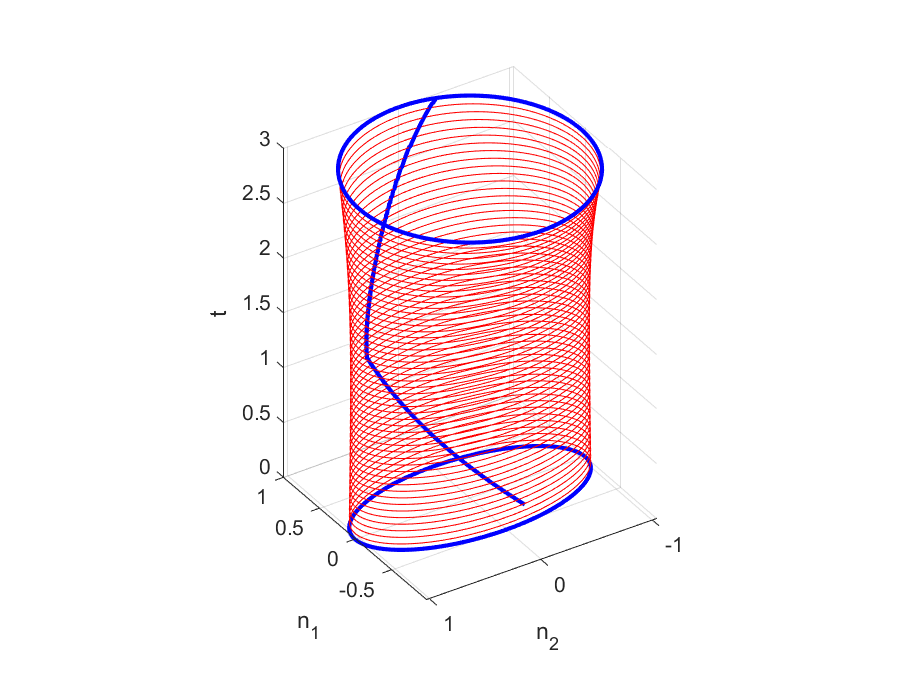
\includegraphics[width = 1.3 \textwidth]{solv_tube.eps}
      \end{figure}
  \end{minipage}
  
\end{frame}

\begin{frame}{Детали численного метода}
\begin{itemize}
    \item Функции \( x^*(t), X_-(t) \) для центра и матрицы конфигурации оценки ищутся с помощью метода Рунге-Кутта четвертого порядка.
    \item Управление выбирается не в виде многозначной функции, а однозначно в виде:
    \begin{equation*}
        u(t,x) = 
        \begin{cases}
            p(t), & \text{если} \ x \in \mathcal{E}_-[t], \\
            p(t) - P(t)l^0(l^0, P(t)l^0)^{-1/2}, & \text{если} \ x \notin \mathcal{E}_-[t],
        \end{cases}
    \end{equation*}
    \item Траектория ищется итерационно из разностного уравнения:
        \begin{equation*}
            x(t_{k+1}) - x(t_k) = h(u(t_k, x(t_k)) + v(t_k)), \quad h = t_{k+1} - t_k.
        \end{equation*}
    \item Значение лагранжевого множителя \( \lambda \) также ищется итерационно среди \( \lambda > 0 \) в силу свойств функции \( f \).
\end{itemize}
    
\end{frame}

\begin{frame}{Список литературы}
    \begin{thebibliography}{0}
	\bibitem{lin_dif_chasing} Понтрягин~Л.\,С.
	\emph{Линейные дифференциальные игры преследования}, \emph{Матем. сб.}, 1980, том 112(154), номер 3(7), 307-330
	
	\bibitem{ellips_calculus} Kurzhanki~A.\,B., \ Vâlyi~I.
	\emph{Ellipsoidal calculus for estimation and control}, \emph{Boston: Birkhäuser}, 1996
	
	\bibitem{dyn_contr_traj_tubes}
	Kurzhanski~A.\,B., \ Varaiya~P. \emph{Dynamics and Control of Trajectory Tubes. Theory and Computation.} \emph{Springer}, 2014
	
\end{thebibliography}
\end{frame}

\end{document}